%\documentclass{beamer}
\documentclass[aspectratio=169]{beamer}
\usetheme{Boadilla}
%\usetheme{Warsaw}
%\setbeamercovered{transparent}
\beamertemplatetransparentcoveredhigh
\usepackage[portuges]{babel}
\usepackage[utf8]{inputenc}
\usepackage{lmodern}
\usepackage[T1]{fontenc}
\usepackage{listings}
\usepackage{hyperref} 
\usepackage[portuguese, linesnumbered, vlined, titlenumbered, ruled]{algorithm2e}
\lstset{frame=tb,
  language=C,
  aboveskip=3mm,
  belowskip=3mm,
  showstringspaces=false,
  columns=flexible,
  basicstyle={\small\ttfamily},
  numbers=none,
  breaklines=true,
  breakatwhitespace=true,
  tabsize=3
}

\newcommand{\eng}[1]{\textsl{#1}}
\newcommand{\cod}[1]{\texttt{#1}}

\title[Análise Assintótica de Algoritmos]{Algoritmos e Estrutura de Dados II}
\subtitle{Análise Assintótica de Algoritmos}
\author[Frederico Santos de Oliveira]{prof. Frederico Santos de Oliveira}
\institute[UFMT]{Universidade Federal de Mato Grosso\\ Instituto de Engenharia}
\date{}

\begin{document}

%%%%%%%%%%%%%%%%%%%%%%%%%%%%%%%%%%%%%%%%%%%%%%%%%%%%%%%%%%%%%%%%%%%%%%%%%%%%%%%%%%%%%%%%%%%%
\begin{frame}[plain]
  \titlepage
\end{frame}

%%%%%%%%%%%%%%%%%%%%%%%%%%%%%%%%%%%%%%%%%%%%%%%%%%%%%%%%%%%%%%%%%%%%%%%%%%%%%%%%%%%%%%%%%%%%
%\section*{Roteiro}
%%%%%%%%%%%%%%%%%%%%%%%%%%%%%%%%%%%%%%%%%%%%%%%%%%%%%%%%%%%%%%%%%%%%%%%%%%%%%%%%%%%%%%%%%%%%

\begin{frame}
  \frametitle{Agenda}
  \tableofcontents
\end{frame}

%%%%%%%%%%%%%%%%%%%%%%%%%%%%%%%%%%%%%%%%%%%%%%%%%%%%%%%%%%%%%%%%%%%%%%%%%%%%%%%%%%%%%%%%%%%%
\section{Introdução}
%%%%%%%%%%%%%%%%%%%%%%%%%%%%%%%%%%%%%%%%%%%%%%%%%%%%%%%%%%%%%%%%%%%%%%%%%%%%%%%%%%%%%%%%%%%%

\begin{frame}{Introdução}
\begin{itemize}
 \item Na última aula aprendemos a calcular a complexidade de um algoritmo contando o nº de vezes que as instruções são executadas.
 \item No entanto, é inviável medir a complexidade exata de um algoritmo, visto que alguns outros fatores podem influenciar nessa complexidade.
 \begin{itemize}
 \item Linguagem de programação
 \item Compilador
 \item Hardware
 \end{itemize}
 \item Precisamos saber a {\bf complexidade assintótica} definida pelo termo dominante de uma função de crescimento.
\end{itemize}
\end{frame}

%%%%%%%%%%%%%%%%%%%%%%%%%%%%%%%%%%%%%%%%%%%%%%%%%%%%%%%%%%%%%%%%%%%%%%%%%%%%%%%%%%%%%%%%%%%%

\begin{frame}{Introdução}{Comparação algoritmo MaxMin}
Ao analisar valores grandes de $n$ percebe-se que as constantes faze pouca diferença...
\begin{table}[]
\centering
\caption{Comparativo MaxMin}
\label{Comparativo2 MaxMin}
\begin{tabular}{c|ccc}
Algoritmo  &  Melhor Caso  &  Pior Caso  &  Caso Médio  \\
\hline
MinMax1  &   4n       &       4n   &  4n \\
MinMax2  &   3n+1     &       5n-1   &  $\frac{(7n -1)}{2}$ \\
MinMax3  &   3n+6     & 4n+4    &  $\frac{7n}{2}$+4 \\
MinMax4  &   3n+1     &      4n-3 &  $\frac{7n}{2}-2$ \\
\end{tabular}
\end{table}
\end{frame}

%%%%%%%%%%%%%%%%%%%%%%%%%%%%%%%%%%%%%%%%%%%%%%%%%%%%%%%%%%%%%%%%%%%%%%%%%%%%%%%%%%%%%%%%%%%%

\begin{frame}{Introdução}
\begin{block}{Comportamento Assintótico}
Quando observamos tamanhos de entrada grandes o suficiente para tornar relevante apenas a ordem de crescimento do tempo de execução, estamos estudando a {\bf eficiência assintótica} dos algoritmos (Cormen et al., 2009).
\end{block}
\begin{itemize}
\item Na notação assintótica, representa-se uma função pelo termo que cresce mais rapidamente, ignorando fatores constantes. 
\item Analisa-se o algoritmo quando o valor tende ao {\it infinito}.
\item Permite ``simplificar'' expressões, focando apenas nas {\bf ordens de grandeza}.
\end{itemize}
\end{frame}

%%%%%%%%%%%%%%%%%%%%%%%%%%%%%%%%%%%%%%%%%%%%%%%%%%%%%%%%%%%%%%%%%%%%%%%%%%%%%%%%%%%%%%%%%%%%

\begin{frame}{Introdução}
Exemplo: Qual os termos dominates das equações a seguir:
\begin{itemize}
\item $T_1(n) = \frac{1}{2} n^2 - 3n$
\item $T_2(n) = n + 1$
\item $T_3(n) = n^5 + n^3 + 100$
\item $T_4(n) = 2^n - \frac{2}{3} n^3 + 5 n^2 - 3 n + 5000$
\item $T_5(n) = \sqrt{ n } + 1$
\item $T_6(n) = n \log_2 n + 2n - 5$
\end{itemize}

\begin{block}{Relações de Domínio}
\begin{equation}
n! \ggg 2^n  \ggg n^3 \ggg n^2 \ggg n \log n \ggg n \ggg log n \ggg 1 \nonumber
\end{equation}
\end{block}

\end{frame}

%%%%%%%%%%%%%%%%%%%%%%%%%%%%%%%%%%%%%%%%%%%%%%%%%%%%%%%%%%%%%%%%%%%%%%%%%%%%%%%%%%%%%%%%%%%%

\begin{frame}{Introdução}
Exemplo: Qual os termos dominates das equações a seguir:
\begin{itemize}
\item $T_1(n) = \frac{1}{2} n^2 - 3n$ 
\begin{itemize}
\item Resposta: $n^2$
\end{itemize}
\item $T_2(n) = n + 1$  
\begin{itemize}
\item Resposta: $n$
\end{itemize}
\item $T_3(n) = n^5 + n^3 + 100$  
\begin{itemize}
\item Resposta: $n^5$
\end{itemize}
\item $T_4(n) = 2^n - \frac{2}{3} n^3 + 5 n^2 - 3 n + 5000$  
\begin{itemize}
\item Resposta: $2^n$
\end{itemize}
\item $T_5(n) = \sqrt{ n } + 1$
\begin{itemize}
\item Resposta: $\sqrt{n}$
\end{itemize}
\item $T_6(n) = n \log_2 n  + 2n - 5$
\begin{itemize}
\item Resposta: $n \log_2 n$
\end{itemize}
\end{itemize}
\end{frame}

%%%%%%%%%%%%%%%%%%%%%%%%%%%%%%%%%%%%%%%%%%%%%%%%%%%%%%%%%%%%%%%%%%%%%%%%%%%%%%%%%%%%%%%%%%%%

\begin{frame}{Introdução}
Utiliza-se uma notação específica:
\begin{itemize}
\item Notação $O$
\begin{itemize}
\item Representa um limite superior, relacionado ao {\bf pior caso}. 
\end{itemize}
\item Notação $\Omega$
\begin{itemize}
\item Representa um limite inferior, relacionado ao {\bf melhor caso}.
\end{itemize}
\item Theta: $\Theta$
\begin{itemize}
\item Representa casos em que os {\bf limites superiores e inferiores são iguais}.
\end{itemize}
\end{itemize}
\end{frame}

%%%%%%%%%%%%%%%%%%%%%%%%%%%%%%%%%%%%%%%%%%%%%%%%%%%%%%%%%%%%%%%%%%%%%%%%%%%%%%%%%%%%%%%%%%%%
\section{Exemplos}
%%%%%%%%%%%%%%%%%%%%%%%%%%%%%%%%%%%%%%%%%%%%%%%%%%%%%%%%%%%%%%%%%%%%%%%%%%%%%%%%%%%%%%%%%%%%

\begin{frame}{Comportamento Assintótico}{BuscaVetor}
Relembrando o tempo de execução do algoritmo que {\bf busca um elemento em um vetor}:
\begin{itemize}
\item Melhor caso: $T(n) = 3$. 
\begin{itemize}
  \item Portanto o algoritmo é $\Omega(1)$.
\end{itemize}
\item Pior caso: $T(n) = 2n + 3$. 
\begin{itemize}
 \item Portanto o algoritmo é $O(n)$
\end{itemize}
\end{itemize}
\end{frame}

%%%%%%%%%%%%%%%%%%%%%%%%%%%%%%%%%%%%%%%%%%%%%%%%%%%%%%%%%%%%%%%%%%%%%%%%%%%%%%%%%%%%%%%%%%%%%

\begin{frame}{Comportamento Assintótico}{MaxVetor}
Relembrando o tempo de execução do algoritmo que encontra o elemento {\bf máximo de um vetor}:
\begin{itemize}
\item Melhor caso: $T(n) = 2n+1$.
\begin{itemize}
\item Portanto o algoritmo é $\Omega(n)$.
\end{itemize}
\item Pior caso: $T(n) = 3n$
\begin{itemize}
\item Portanto o algoritmo é $O(n)$.
\end{itemize}
\item Como o algoritmo é $\Omega(n)$ e $O(n)$, ele também é $\Theta(n)$. 
\end{itemize}
\end{frame}

%%%%%%%%%%%%%%%%%%%%%%%%%%%%%%%%%%%%%%%%%%%%%%%%%%%%%%%%%%%%%%%%%%%%%%%%%%%%%%%%%%%%%%%%%%%%%

\begin{frame}{Comportamento Assintótico}{MaxMin}
Relembre as funções:
\begin{table}[]
\centering
\caption{Comparativo MaxMin}
\begin{tabular}{c|ccc}
Algoritmo  &  Melhor Caso  &  Pior Caso  &  Caso Médio  \\
\hline
MinMax1  &   4n       &       4n   &  4n \\
MinMax2  &   3n+1     &       5n-1   &  $\frac{(7n -1)}{2}$ \\
MinMax3  &   3n+6     & 4n+4    &  $\frac{7n}{2}$+4 \\
MinMax4  &   3n+1     &      4n-3 &  $\frac{7n}{2}-2$ \\
\end{tabular}
\end{table}
\begin{itemize}
 \item Observe que todos os algoritmos tem a mesma complexidade assintótica.
 \item Todos são $O(n)$ e $\Omega(n)$. Portanto, são $\Theta(n)$.
\end{itemize}
\end{frame}

%%%%%%%%%%%%%%%%%%%%%%%%%%%%%%%%%%%%%%%%%%%%%%%%%%%%%%%%%%%%%%%%%%%%%%%%%%%%%%%%%%%%%%%%%%%%%
%
%\begin{frame}
%\begin{itemize}
% \item Quando uma função é melhor que outra?
% \item Se queremos minimizar o tempo, funções de crescimento menor são melhores.
% \item Uma função domina outra se à medida que $n$ cresce ela fica ``infinitamente maior''.
% \item Matematicamente: $f(n) \gg g(n)$ se $\lim_{n \rightarrow \infty} g(n)/f(n) = 0$.
%\end{itemize}
%\begin{block}{Relações de Domínio}
%$n! \gg 2^n \gg n^3 \gg n^2 \gg n \log n \gg n \gg \log n \gg 1$
%\end{block}
%\end{frame}
%
%%%%%%%%%%%%%%%%%%%%%%%%%%%%%%%%%%%%%%%%%%%%%%%%%%%%%%%%%%%%%%%%%%%%%%%%%%%%%%%%%%%%%%%%%%%%%
%
%\begin{frame}{Comportamento Assintótico}
%Se uma operação demorar $10^{-9}$ segundos.
%\begin{figure}[!ht]
%  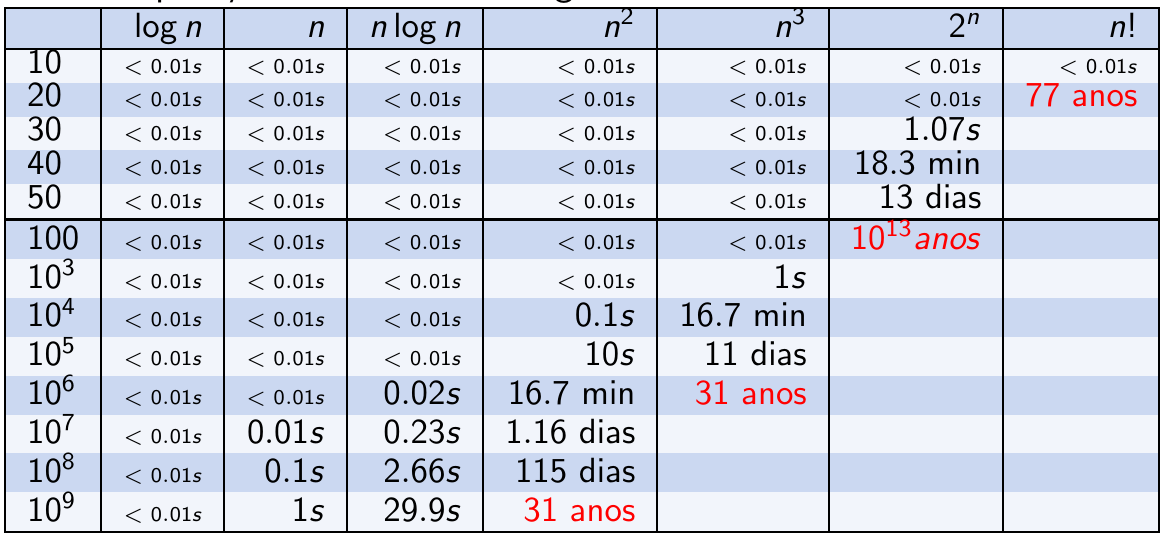
\includegraphics[width=300pt]{imgs/comparativo_tempo_execucao.png}
%\end{figure} 
%\end{frame}
%
%%%%%%%%%%%%%%%%%%%%%%%%%%%%%%%%%%%%%%%%%%%%%%%%%%%%%%%%%%%%%%%%%%%%%%%%%%%%%%%%%%%%%%%%%%%%%
%
%\begin{frame}{Comportamento Assintótico}
%\begin{figure}[!ht]
%  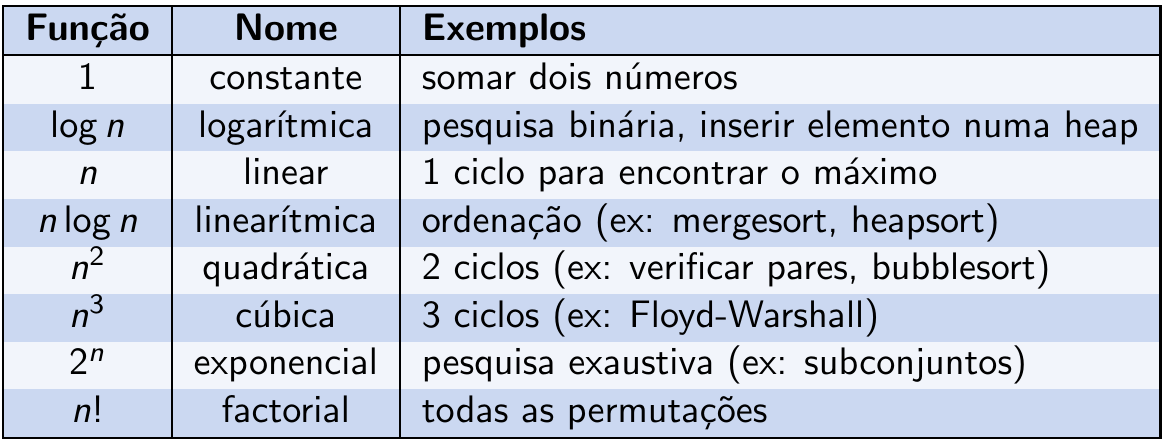
\includegraphics[width=300pt]{imgs/exemplos.png}
%\end{figure} 
%\end{frame}
%%%%%%%%%%%%%%%%%%%%%%%%%%%%%%%%%%%%%%%%%%%%%%%%%%%%%%%%%%%%%%%%%%%%%%%%%%%%%%%%%%%%%%%%%%%%
\section{Classes Assintóticas}
%%%%%%%%%%%%%%%%%%%%%%%%%%%%%%%%%%%%%%%%%%%%%%%%%%%%%%%%%%%%%%%%%%%%%%%%%%%%%%%%%%%%%%%%%%%%

\begin{frame}{Classes Assintóticas}
\begin{itemize}
 \item Em geral, é interessante agrupar os algoritmos/problemas em {\bf Classes de Comportamento Assintótico}.
 \item Quando dois algoritmos fazem parte da mesma classe de comportamento assintótico, eles são ditos equivalentes
 
\end{itemize}
\end{frame}

%%%%%%%%%%%%%%%%%%%%%%%%%%%%%%%%%%%%%%%%%%%%%%%%%%%%%%%%%%%%%%%%%%%%%%%%%%%%%%%%%%%%%%%%%%%%

\begin{frame}{Classes Assintóticas}{$O(1)$}
$T(n) = O(1)$
\begin{itemize}
 \item Algoritmos de complexidade $O(1)$ são ditos de {\bf complexidade constante}.
 \item Uso do algoritmo independe de $n$.
 \item As instruções do algoritmo são executadas um número fixo de vezes
 \end{itemize}
\end{frame}

%%%%%%%%%%%%%%%%%%%%%%%%%%%%%%%%%%%%%%%%%%%%%%%%%%%%%%%%%%%%%%%%%%%%%%%%%%%%%%%%%%%%%%%%%%%%

\begin{frame}{Classes Assintóticas}{$O(\log n)$}
$T(n) = O(\log n)$
\begin{itemize}
 \item Um algoritmo de complexidade $O(\log n)$ é dito ter {\bf complexidade logarítmica}.
 \item Típico em algoritmos que transformam um problema em outros menores.
 \item Pode-se considerar o tempo de execução como menor que uma constante grande.
 \begin{itemize}
 \item Quando $n=10^3$, $\log_{2} n \approx 10$; quando $n = 10^6$, $\log_2 n \approx 20$.
 \item Para dobrar o valor de $\log n$ temos de considerar o quadrado de $n$.
 \item A base do logaritmo muda pouco estes valores: quando $n=10^3$, $\log_2 n \approx 20$ e $\log_{10} n$ é 6.
 \end{itemize}
 \end{itemize}
\end{frame}

%%%%%%%%%%%%%%%%%%%%%%%%%%%%%%%%%%%%%%%%%%%%%%%%%%%%%%%%%%%%%%%%%%%%%%%%%%%%%%%%%%%%%%%%%%%%

\begin{frame}{Classes Assintóticas}{$O(n)$}
$T(n) = O(n)$
\begin{itemize}
 \item Um algoritmo de complexidade O(n) é dito ter complexidade linear.
 \item Em geral, um pequeno trabalho é realizado sobre cada elemento de entrada.
 \item É a melhor situação possível para um algoritmo que tem de processar/produzir $n$ elementos de entrada/saída.
 \item Cada vez que ndobra de tamanho, o tempo de execução dobra
 \end{itemize}
\end{frame}

%%%%%%%%%%%%%%%%%%%%%%%%%%%%%%%%%%%%%%%%%%%%%%%%%%%%%%%%%%%%%%%%%%%%%%%%%%%%%%%%%%%%%%%%%%%%

\begin{frame}{Classes Assintóticas}{$O(n \log n)$}
$T(n) = O(n \log n)$
\begin{itemize}
 \item Típico em algoritmos que quebram um problema em outros menores, resolvem cada um deles independentemente e ajuntando as soluções depois.
 \item Quando $n=1$ milhão, $n\log_2 n \approx 20$ milhões.
 \item Quando $n=2$ milhões, $n\log_2 n$ é cerca de 42 milhões, pouco mais do que o dobro.
 \end{itemize}
\end{frame}


%%%%%%%%%%%%%%%%%%%%%%%%%%%%%%%%%%%%%%%%%%%%%%%%%%%%%%%%%%%%%%%%%%%%%%%%%%%%%%%%%%%%%%%%%%%%

\begin{frame}{Classes Assintóticas}{$O(n^2)$}
$T(n) = O(n^2)$
\begin{itemize}
 \item Um algoritmo de complexidade $O(n^2)$ é dito ter {\bf complexidade quadrática}.
 \item Ocorrem quando os itens de dados são processados aos pares, muitas vezes em um anel dentro de outro.
 \item Quando $n$ é mil, o número de operações é da ordem de 1 milhão.
 \item Sempre que $n$ dobra, o tempo de execução é multiplicado por 4.
 \item Úteis para resolver problemas de tamanhos relativamente pequenos.
 \end{itemize}
\end{frame}

%%%%%%%%%%%%%%%%%%%%%%%%%%%%%%%%%%%%%%%%%%%%%%%%%%%%%%%%%%%%%%%%%%%%%%%%%%%%%%%%%%%%%%%%%%%%

\begin{frame}{Classes Assintóticas}{$O(n^3)$}
$T(n) = O(n^3)$
\begin{itemize}
 \item Um algoritmo de complexidade $O(n^3)$ é dito ter {\bf complexidade cúbica}.
 \item Úteis apenas para resolver pequenos problemas.
 \item Quando $n=100$, o número de operações é da ordem de 1 milhão.
 \item Sempre que $n$ dobra, o tempo de execução fica multiplicado por 8.
 \end{itemize}
\end{frame}

%%%%%%%%%%%%%%%%%%%%%%%%%%%%%%%%%%%%%%%%%%%%%%%%%%%%%%%%%%%%%%%%%%%%%%%%%%%%%%%%%%%%%%%%%%%%

\begin{frame}{Classes Assintóticas}{$O(2^n)$}
$T(n) = O(2^n)$
\begin{itemize}
 \item Um algoritmode complexidade $O(2^n)$ é dito ter {\bf complexidade exponencial}.
 \item Geralmente não são úteis sob o ponto de vista prático.
 \item Ocorrem na solução de problemas quando se usa força bruta para resolvê-los.
 \item Quando $n=20$, o tempo de execução é cercade 1 milhão. Quando $n$ dobra, o tempo fica elevado ao quadrado.
 \end{itemize}
\end{frame}


%%%%%%%%%%%%%%%%%%%%%%%%%%%%%%%%%%%%%%%%%%%%%%%%%%%%%%%%%%%%%%%%%%%%%%%%%%%%%%%%%%%%%%%%%%%%

\begin{frame}{Classes Assintóticas}{$O(n!)$}
$T(n) = O(n!)$
\begin{itemize}
 \item Um algoritmode complexidade $O(n!)$ é dito ter {\bf complexidade exponencial}, apesar de $O(n!)$ ter comportamento muito pior do que $O(2^n)$.
 \item Geralmente ocorrem quando se usa força bruta para solução do problema.
 \item Ocorrem na solução de problemas quando se usa força bruta para resolvê-los.
 \item $n=20$ $\rightarrow$ $20! = 2432902008176640000$, um número com 19 dígitos.
 \item $n=40$ $\rightarrow$ um número com 48 dígitos.
 \end{itemize}
\end{frame}


%%%%%%%%%%%%%%%%%%%%%%%%%%%%%%%%%%%%%%%%%%%%%%%%%%%%%%%%%%%%%%%%%%%%%%%%%%%%%%%%%%%%%%%%%%%%%

\begin{frame}{Comportamento Assintótico}
\begin{figure}[!ht]
  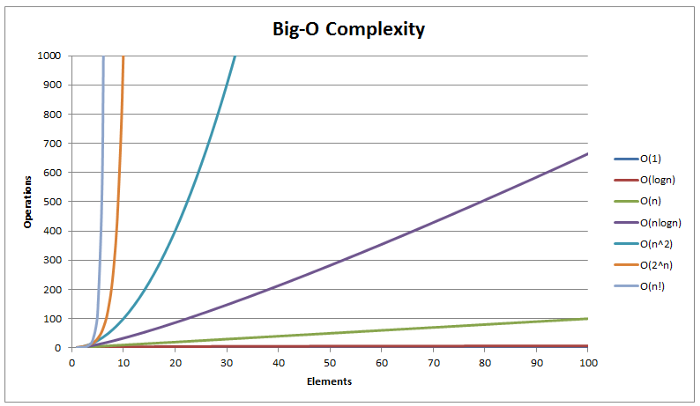
\includegraphics[width=300pt]{imgs/comparativo_complexidade.png}
\end{figure} 
\end{frame}

%%%%%%%%%%%%%%%%%%%%%%%%%%%%%%%%%%%%%%%%%%%%%%%%%%%%%%%%%%%%%%%%%%%%%%%%%%%%%%%%%%%%%%%%%%%%

\begin{frame}
  \frametitle{FIM}
\centering
\alert{Fim}
\end{frame}	

%%%%%%%%%%%%%%%%%%%%%%%%%%%%%%%%%%%%%%%%%%%%%%%%%%%%%%%%%%%%%%%%%%%%%%%%%%%%%%%%%%%%%%%%%%%%

\begin{frame}[plain]
  \titlepage
\end{frame}

%%%%%%%%%%%%%%%%%%%%%%%%%%%%%%%%%%%%%%%%%%%%%%%%%%%%%%%%%%%%%%%%%%%%%%%%%%%%%%%%%%%%%%%%%%%%

\end{document}
